\subsection{Электрический диполь. Распределение напряженности и потенциала. Дипольный момент. силы, действующие на диполь во внешнем поле}

\begin{definition}
    Электрический диполь — система двух одинаковых по величине и противоположных по знаку точечных зарядов $+q$ и $-q$. 
\end{definition}

\begin{definition}
    Точечный диполь — если расстояние $l$ между зарядами значительно меньше расстояния $r$ до точки, где рассматривается поле, создаваемое этими зарядами.
\end{definition}

\begin{definition}
    Плечо диполя — вектор $\vec l$, направленный от отрицательного заряда к положительному
\end{definition}

\begin{definition}
    Дипольный момент — вектор $\vec{p} = q\vec{l}$
\end{definition}

$$\varphi=k\bigg(\frac{q}{r_1}-\frac{q}{r_2}\bigg)=kq\bigg(\frac{1}{r_1}-\frac{1}{r_2}\bigg)$$

где $r_1$ - расстояние от положительного заряда до точки наблюдения,
$r_2$ - расстояние от отрицательного заряда до точки наблюдения,
$k$ - постоянная Больцмана.

\begin{remark}
    Потенциал через момент:

    $$\varphi=k\frac{qd\cos\alpha}{r^2}=k\frac{p\cos\alpha}{r^2}$$
\end{remark}

\begin{remark}
    Потенциал через вектора:

    $$\varphi=k\frac{pr\cos\alpha}{r^3}=k\frac{(\vec p,\ \vec r)}{r^3}$$
\end{remark}

По формуле $E=-grad\varphi$ можно определить поле диполя $E$, пользуясь сферической системой координат:

$$\overline E=-grad\varphi=-\bigg(\overline r_0\frac{\partial\varphi}{\partial r}+ \overline \theta_0\frac{\partial\varphi}{r\ \partial \theta}+\overline\alpha_0\frac{\partial\varphi}{r\sin\theta\ \partial\alpha} \bigg)$$

получаем

$$\overline E=\frac{ql}{4\pi\epsilon r^3}(\overline r_02\cos\theta+\overline\theta_0\sin\theta)$$

Поле диполя симметрично относительно его оси. Силовые линии поля в меридиональной плоскости:

\begin{figure}[h]
    \centering
    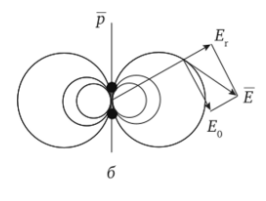
\includegraphics[width=0.3\linewidth]{imgs/q20i1.png}
\end{figure}

Диполь во внешнем электрическом поле.

\begin{figure}[h]
    \centering
    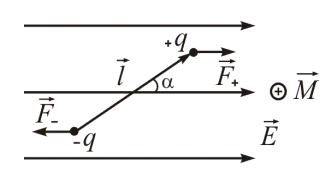
\includegraphics[width=0.3\linewidth]{imgs/q20i2.png}
\end{figure}

В однородном электрическом поле вектор напряженности имеет одно и то же направление в любой точке, 
и на диполь будут действовать силы $F_+$ и $F_-$. Эти силы равны по модулю: $F_+=F_-=qE$ и противоположны по направлению. 
Они образуют пару сил, плечо которой равно $l\sin\alpha$. 

Модуль момента этой пары сил равен произведению силы и плеча: $M=qEl\sin\alpha=PE\sin\alpha$ или в векторном виде 
$\vec M=\vec P\times\vec E$.

При повороте на угол $\alpha$ энергия диполя изменится на величину:
$$W=\int PE\sin\alpha\ d\alpha=-PE\cos\alpha$$
